\chapter{Implementation in seL4}
\label{chap:implementation}

In the previous chapter we presented our mechanisms for temporal isolation and safe resource sharing
in a high-assurance microkernel. 
Now we delve into the implementation details of scheduling contexts, scheduling context donation,
passive servers, timeout fault handlers, and IPC forwarding in \selfour. First we explore new kernel
objects, followed by new and altered API methods, and finally look at structural changes.

\section{Objects}

We add two new objects to the kernel, \emph{\glspl{SCO}} and \emph{resume objects}. Additionally, we modify
the \gls{TCB} object although do not increase its total size. Finally, we modify the notification
object to allow \glspl{SCO} to allow single-threaded, passive servers to receive signals in
addition to IPC messages.

\subsection{Resume objects}
\label{s:resume}

Resume objects, modelled after KeyKOS~\citep{Bomberger_FFHLS_92}, are a new object type that
generalise ``reply capabilities'' of baseline \selfour introduced in \cref{s:ipc}.  Recall that in
baseline \selfour, the receiver of the message (i.e.\ the server) receives the reply capability in a
magic ``reply slot'' in its capability space. The server replies by invoking that capability. Resume
objects remove the magic by explicitly representing the reply channel, and servers with multiple
clients can dedicate a resume object per client.  Instead of generating a one-shot reply capability
in a reply slot on a \call, the operation populates a resume object, while \recv de-populates the
resume object.  They also provide more efficient support for stateful servers that handle concurrent
client sessions, which we expand on further when we introduce the changed system call \gls{API} in
\cref{s:new-api}.

\begin{table}[b]
    \centering
    \rowcolors{2}{gray!25}{}
    \begin{tabularx}{\textwidth}{lX}\toprule
        \emph{Field} & \emph{Description} \\\midrule
        \code{tcb}    & The calling or waiting thread that is blocked on this reply object. \\
        \code{prev} & \code{NULL} if this is the start of the call stack, otherwise points to the previous
        reply object in the call stack. \\
        \code{next} & Either a pointer to the scheduling context that was last donated using this
        reply object, if this reply object is the head of a call stack (the last caller before the
        server) or a pointer to the next reply object in the stack. 0 if no scheduling context was
        passed along the stack.\\\bottomrule
    \end{tabularx}
    \caption{Fields in a reply object.}
    \label{tab:reply_object}
\end{table}


Resume objects are small (16 bytes on 32-bit platforms, and 32 bytes on 64-bit platforms), and
contain the fields shown in \cref{tab:reply_object}.

There are three states a resume object can be in: idle, meaning it is not currently being used,
waiting, meaning it is being used by a thread blocked and waiting for a message, or active,
which means the resume object currently has a thread blocked waiting for a reply associated with it.

\begin{figure}[t]
    \centering
    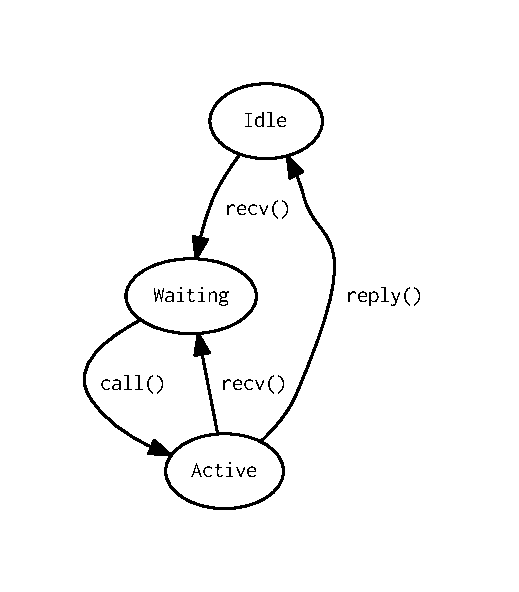
\includegraphics[width=0.6\textwidth]{resume}
    \caption{State diagram of resume objects.}
    \label{f:resume-state-diagram}
\end{figure}

Valid state transitions are shown in \cref{f:resume-state-diagram}. Resume objects are provided to
\recv system calls along with endpoint capabilities, which transitions them from idle to
waiting.
If the endpoint is invoked with a \call, the caller is blocked on the resume capability, and
it transitions to active.  
If a resume object is directly invoked, using a sending system call (recall from
\cref{sec:sel4-system-call-and-invocations} that sending system calls are \send,
\nbsend, \call, \reply) then a reply message is delivered to the thread blocked on
the object. Finally, if a resume object is in an active state, and provided to \recv, the object
is first invoked, and removed from the call stack, which we now examine in detail. 

\subsubsection{The call stack}

Active resume objects track the \emph{call stack} that is built as nested \call operations take
place. A \call triggers to a push operation, adding to the top of the stack, and a reply message a
pop, removing the top of the stack.  The call stack allows us to track the path of a donated
scheduling context, from caller to callee, so that it can be returned to the previous caller
regardless of which thread sends the reply message. This is a direct consequence of flexible resume
capabilities: resume capability can be moved between threads, and \emph{any} thread can execute the
reply: usually the server, but occasionally a timeout fault handler, or a nested server which
received the resume capability via \gls{IPC} forwarding. It is therefore impossible to derive the
original callee from the thread sending the reply message.

The call stack is structured as a doubly-linked list, with one minor difference: the head of the
call stack is the scheduling context that was donated along the stack, which itself contains a
pointer to the thread currently executing on it. Each resume object then forms a node in the
stack, going back to the original caller at the base. The \gls{SCO} remains the head of the stack
until the \gls{SCO} returns to the initial caller and the stack is fully dismantled.  When a reply
message is sent, the scheduling context travels back along the call stack and the head resume object
is popped.  Reply objects also point to the thread which donated the \gls{SCO} along the stack,
allowing the SCO to be returned to that thread when a reply message is sent.  This process is
illustrated in \cref{f:reply-stack}, where $A$ has called $S_{1}$ which has called  $S_{2}$.

\begin{figure}[t]
    \centering
    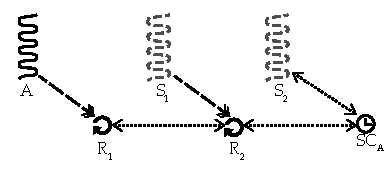
\includegraphics[width=0.7\textwidth]{replychain}
    \caption{The state of the reply stack when a nested server $S_{2}$ is
performing a request on behalf of an initial server $S_{1}$ for client $A$.}
    \label{f:reply-stack}
\end{figure}

In a capability system, one of the biggest challenges is that capabilities can be deleted at any
time. The deletion semantics of the call stack are as follows: 
\begin{itemize}
    \item If the \gls{SCO} is deleted, the head of the call stack becomes the first resume object. To avoid
        a long-running operation, the call stack of resume objects remains linked, and is dismantled
        as each resume object is deleted.
    \item If the head resume object (the object that points to the SC) is deleted, the \gls{SCO} is
        returned along the stack to the caller. 
    \item If a resume object in the middle of the stack is deleted, we use the standard operation to
        remove a node from a doubly-linked list: the previous node is connected to the next node,
        and the deleted object is no longer pointed to by any member of the stack.
    \item If the resume object at the start of the stack, the node corresponding to the initial
        caller, it is simply removed. The \gls{SCO} cannot return to the initial caller by means of a reply
        message.
\end{itemize}
    
\subsection{Scheduling context objects}
\label{s:sco}

We introduce a new kernel object type, \glspl{SCO}, which all processing time is accounted against, 
and a new scheduler invariant: any thread in the scheduler must have a \gls{SCO}. 
\glspl{SCO} are variable sized objects that represent access to a certain amount of time and
consist of a core amount of fields, and a circular buffer to track the consumption of time.
Scheduling contexts encapsulate processor time reservations,
derived from sporadic task parameters: minimum inter-arrival time ($T$) and a set of replenishments which is
populated from an original execution budget ($C$), representing the reserved rate
($U$) = $\frac{C}{T}$.
Fields in an \glspl{SCO} are shown in \cref{t:sc-fields}.

\begin{table}[t] 
    \centering
    \rowcolors{2}{gray!25}{}
    \begin{tabularx}{\textwidth}{lX}\toprule
        \emph{Field}   & \emph{Description}\\\midrule
        \code{Period}  & The replenishment period, $T$. \\
     \code{Consumed} & The amount of cycles consumed since the last reset. \\
     \code{Core}     & The ID of the processor this scheduling context grants time on.\\
     \code{TCB}      & A pointer to the thread (if any) that this scheduling context is
        currently providing time to.\\
     \code{Reply}    & A pointer to the last resume object in a call stack
        which this \gls{SCO} was donated along.\\
     \code{Notification} & A pointer (if any) to the notification object this \gls{SCO} is bound
        to.\\
     \code{Badge} & A unique identifier for this scheduling context, which is delivered as part of a
        timeout fault message to identify the faulting client.\\
     \code{YieldFrom} & Pointer to a \gls{TCB} that has performed a directed yield to this
        \gls{SCO}.\\
     \code{Head,Tail} & Indexes to the circular buffer of sporadic replenishments.\\
     \code{Max} & Size of the circular buffer of replenishments for this scheduling context.\\
        \bottomrule
    \end{tabularx}
    \caption{Fields of a scheduling context object.}
    \label{t:sc-fields}
\end{table}

\subsubsection{Replenishments}

In addition to the core fields, \glspl{SCO} contain a variable amount of \emph{replenishments},
which consist of a \code{timestamp} and \code{amount}. These are used for both round-robin and
sporadic threads. For round-robin threads we simply use the head replenishment to track how much
time is left in that \glspl{SCO} timeslice. 

Sporadic threads are more complex; the replenishments form a circular buffer used to track 
how much time a thread can execute for (\code{amount}) and when that time can be used (\code{timestamp}).
The size of the circular buffer is limited by both a variable
provided on configuration and the size of the \gls{SCO}, configured on creation. This allows system
designers to control the preemption and fragmentation of sporadic replenishments as discussed in
\cref{sec:model-sporadic}. 

Each \gls{SCO} is minimum $2^{8}$ bytes in size, which can hold eight or ten replenishments for 32
and 64-bit processors respectively. This is sufficient for most uses, but more replenishments can
be supported by larger sizes, allowing system designers to trade-off latency for fragmentation
overhead in the sporadic server implementation. Scheduling contexts can be created as larger
objects, as any power of two, then the rest of the object can be filled with replenishments, as
shown in \cref{t:impl-sc-layout}. System designers can then use the \code{max} replenishment field
to specify exact the number of replenishment to use, up to the object size. 

\begin{table}[t] 
    \centering
    \begin{tabular}{c|c|c|c|c|}\cline{2-5}
        0x00 &  \multicolumn{2}{c}{\texttt{period}} & \multicolumn{2}{|c|}{\texttt{consumed}}
        \\\cline{2-5}
        0x10 & \texttt{core}                         & \texttt{TCB} & \texttt{reply} & \texttt{ntfn} \\\cline{2-5}
        0x20 &\texttt{badge}                        & \texttt{yieldFrom}                               & \texttt{head}  & \texttt{tail} \\\cline{2-5}
        0x30 & \texttt{max}                          &                                                  &                & \\\cline{2-5}
        0x40 & \multicolumn{4}{c|}{\texttt{replenishment$_{0}$}}  \\\cline{2-5}
        0x50 & \multicolumn{4}{c|}{\texttt{replenishment$_{1}$}}  \\\cline{2-5}
        \ldots & \multicolumn{4}{c|}{\ldots}  \\\cline{2-5}
        0xF0 & \multicolumn{4}{c|}{\texttt{replenishment$_{n}$}}  \\\cline{2-5}


    \end{tabular}
    \caption{Layout of a scheduling context object on a 32-bit system.}
    \label{t:impl-sc-layout}
\end{table}

\subsubsection{Admission}

Like any \selfour object, scheduling contexts are created from zeroed, untyped memory. Consequently,
new scheduling objects do not grant authority to any processing time at all, as the parameters are
all set to zero. To configure a scheduling context, the new \schedcontrol capability must be
invoked, which allows the period, initial sporadic replenishment, maximum number of refills, and
badge fields to be set. The processing core is derived from the \schedcontrol capability
that is invoked: only one exists per core. 

The \schedcontrolconfigure operation behaves differently depending on the state of the target scheduling
context and can be used not only to configure \glspl{SCO} but to migrate threads across cores, and
change the available bandwidth of a currently runnable thread. Semantics are as follows:

\begin{itemize}
\item If the scheduling context is not bound
to a currently runnable thread, or does not represent any time currently, the operation is 
a basic configure: the fields are
simply set and the first replenishment is configured with budget provided and timestamp of the
kernel entry. The function \code{refill\_new} is used to \cref{list:refill-init}
\item If the scheduling context is bound to a currently runnable thread, but that scheduling
context is for a different processing core than the \schedcontrol capability, the fields are
set and the thread is migrated to the new core.  
\item Finally, if the scheduling context is bound to a currently running thread and the
    \schedcontrol capability is for the same core, we update the replenishment list without
    allowing the sliding window constraint to be violated. The function \code{refill\_update} shows the
    algorithm used.
\end{itemize}

\begin{listing}[h!]
\begin{minted}{c}
/* Short hand for accessing refill queue items */
#define REFILL_INDEX(sc, index) (((refill_t *) ((word_t) (sc) + sizeof(sched_context_t)))[index])
#define REFILL_HEAD(sc) REFILL_INDEX((sc), (sc)->head)
#define REFILL_TAIL(sc) REFILL_INDEX((sc), (sc)->tail)

void refill_new(sched_context_t *sc, word_t max_refills, ticks_t budget, ticks_t period)
{
    sc->period = period;
    sc->head = 0;
    sc->tail = 0;
    sc->max = max_refills;
    /* full budget available */
    REFILL_HEAD(sc).amount = budget;
    /* budget can be used from now */
    REFILL_HEAD(sc).time = current_time;
}

void refill_update(sched_context_t *sc, ticks_t new_period, ticks_t new_budget, word_t new_max_refills)
{
    /* move the head refill to the start of the list */
    REFILL_INDEX(sc, 0) = REFILL_HEAD(sc);
    sc->head = 0;
    /* truncate refill list to size 1 */
    sc->tail = sc->head;
    sc->max = new_max_refills;
    sc->period = new_period;

    if (REFILL_HEAD(sc).time < current_time) {
        REFILL_HEAD(sc).time = current_time;
    }

    if (REFILL_HEAD(sc).amount >= new_budget) {
        /* if the heads budget exceeds the new budget just trim it */
        REFILL_HEAD(sc).amount = new_budget;
    } else {
        /* otherwise schedule the rest for the next period */
        refill_t new = { .amount = (new_budget - REFILL_HEAD(sc).amount),
                         .time = REFILL_HEAD(sc).time + new_period
                       };
        refill_add_tail(sc, new);
    }
}
\end{minted}
\caption{Code to initialise a scheduling context that is not bound to a currently active thread.}
\label{list:refill-init}
\end{listing}

\subsubsection{Sporadic Servers}
\label{sec:impl-sporadic}

Configured scheduling contexts with zero extra refills behave like polling servers (\cref{p:polling-servers}),
otherwise they behave as sporadic servers (\cref{p:sporadic}), allowing application developers to
tune the behaviour of threads depending on their preemption levels and execution durations.

The algorithms to manage replenishments are taken from \citet{Danish_LW_11}, with adjustments to
support periods of 0 (for round robin threads) and to implement a minimum budget.  Whenever the
current scheduling context is changed, \texttt{check\_budget} as shown in Listing
\ref{list:check-budget} is called to bill the amount of time consumed since the last scheduling
context change.  `check\_budget` If the budget is not completely consumed by \texttt{check\_budget},
\texttt{split\_budget} as shown in Listing \ref{list:split-check} is called to schedule the
subsequent refill for the chunk of time just consumed.  If the replenishment buffer is full, or the
amount consumed is less than the minimum budget, the amount used is merged into the next
replenishment.  When a new scheduling context is switch to, \texttt{unblock\_check} 
(\ref{list:unblock-check}) is used, which merges any replenishments that are already available,
avoiding unnecessary preemptions.

\begin{listing}[h]
\begin{minted}{c}
uint_64_t check_budget(sched_context_t *sc, uint64_t usage) {
  while (REFILL_HEAD(sc).amount <= usage) {
    // exhaust and schedule replenishment
    old_head = pop_head(sc);
    usage -= old_head.amount;
    old_head.time += sc->period;
    add_tail(sc, old_head)
  }
  // handle budget overrun
  if (usage > 0 && sc->period > 0) {
    // delay refill by overrun
    REFILL_HEAD(sc).time += usage;
    // merge replenishments if time overlaps
    if (refill_size(sc) > 1 && REFILL_HEAD(sc).time + REFILL_HEAD(sc).amount >= refill_next(sc).time) {
      refill_t old_head = pop_head(sc);
      REFILL_HEAD(sc).amount += old_head.amount;
    }
  }
}
\end{minted}
\caption{Check budget routine used to implement sporadic servers.}
\label{list:check-budget}
\end{listing}

\begin{listing}[h]
\begin{minted}{c}
void split_check(sched_context_t *sc, uint64_t usage) {
  uint64_t remnant = REFILL_HEAD(sc).amount - usage;
  if (remnant < MIN_BUDGET && refill_size(sc) == 1) {
    // delay entire replenishment refill too small to use and nothing to merge with
    REFILL_HEAD(sc).time += sc->period;
    return;
  }
  if (refill_size(sc) == sc->refill_max || remnant < MIN_BUDGET) {
    // merge remnant - out of space or its too small
    pop_head(sc);
    REFILL_HEAD(sc).amount += remant;
  } else {
    // split the head refill
    REFILL_HEAD(sc).amount = remnant;
  }
  // schedule the used amount
  refill_t split;
  split.amount = usage;
  split.time = REFILL_HEAD(sc).time + sc->period;
  add_tail(sc, split);
}
\end{minted}
\caption{Split check routine used to implement sporadic servers.}
\label{list:split-check}
\end{listing}


\begin{listing}[h]
\begin{minted}{c}
void unblock_check(sched_context_t *sc) {
  if (!REFILL_HEAD(sc).time > current_time)) {
    return;
  }
  REFILL_HEAD(sc).time = current_time;
  // merge available replenishments
  while (refill_size(sc) > 1) {
    if (refill_next(sc).time < current_time + REFILL_HEAD(sc).amount) {
      refill_t old_head = pop_head(sc);
      REFILL_HEAD(sc).amount += old_head.amount;
      REFILL_HEAD(sc).time = current_time;
    } else {
      break;
    }
    if (REFILL_HEAD(sc).amount < MIN_BUDGET) {
      // second part of split_check can leave refills with less than MIN_BUDGET amount, detect them here and merge.
      refill_t old_head = pop_head(sc);
      REFILL_HEAD(sc).amount += old_head.amount;
    }
}
\end{minted}
\caption{Unblock check routine used to implement sporadic servers.}
\label{list:unblock-check}
\end{listing}

\subsection{Thread control blocks}

Recall from \cref{sec:sel4-tcb} that \glspl{TCB} are the abstraction of an execution context in
\selfour, which are formed from a TCB data structure and a CNode containing capabilities specific to
that thread. We make several alterations to this structure, but do not impact the \gls{TCB} size, as
there was enough space available. The altered fields are shown in \cref{t:tcb-fields}.

\begin{table}[b] 
    \centering
    \rowcolors{2}{gray!25}{}
    \begin{tabularx}{\textwidth}{lX}\toprule
        \emph{Field}   & \emph{Description}\\\midrule
        \sout{\code{timeslice}} & Used to track the timeslice, replaced by the scheduling context. \\
        \code{scheduling context} & The scheduling context (if any) this \gls{TCB} consumes time from. \\
        \code{MCP} & The \gls{MCP} of this \gls{TCB}. \\
        \code{reply} & A pointer to the resume object this TCB is blocked on, if the TCB is
        \code{BlockedOnReply} or \code{BlockedOnRecv}. \\
        \code{yieldTo} & Pointer to the \gls{SCO} this \gls{TCB} has performed a directed yield to,
        if any.\\
        \sout{\code{faultEndpoint}} &  Moved to the TCB CNode. \\
        \bottomrule
    \end{tabularx}
    \caption{Added and removed fields in a \gls{TCB} object.}
    \label{t:tcb-fields}
\end{table}


\subsubsection{Fault endpoints}

We also change the contents of the TCB CNode, removing two slots previously required by the reply
capability implementation, as resume objects are now provided to receiving system calls, and
no slot in the TCB CNode is required. Additionally, we change the behaviour of fault handlers: in
baseline seL4, the fault handling cap is looked up on every single fault, increasing the overhead of
fault handling. To minimise this overhead, we look up the fault endpoint when it is configured, and
install it in the TCB CNode. We do the same for timeout fault endpoints. 

\subsubsection{Maximum controlled priorities}

The MCP, or \emph{maximum controlled priority}, resurrects a concept from early L4
kernels~\citep{Liedtke_96:rm}. It supports lightweight, limited manipulation of thread priorities,
useful e.g.\ for implementing user-level thread packages. When setting
the priority or MCP of a TCB, \(A\),
the caller must provide the capability to a TCB, \(B\), (which could be the caller's
TCB). The caller is allowed to set the priority or MCP of \(A\) up to the value
of \(B\)'s MCP.\footnote{Obviously, this operation also requires a capability to \(A\)'s TCB.}
In a typical system, most threads
will run with an MCP of zero and have no access to TCB capabilities with a higher MCP, meaning they
cannot raise any thread's priority.
The MCP is taken from an explicitly-provided TCB, rather than the caller's, to avoid the
confused deputy problem~\citep{Hardy_88}.

\subsection{Notification objects}

A scheduling context object can be associated with notification object, which allows a passive
server with bound notifications to receive signals and run on the notification's
scheduling context to process those signals.
We add a pointer to the scheduling context from the notification context, as well as vice-versa, to 
facilitate this mechanism, which increases the size of the notification object from $2^{4}$ to
$2^{5}$ on 32-bit, and $2^{5}$ to $2^{6}$ on 64-bit. 

\section{MCS API}
\label{s:new-api}

We now present the new \gls{MCS} API for \selfour, which alters the core system call API, 
as well as adding new invocations and modifying existing ones. In this section we also
present the semantics of scheduling context donation, which are directly linked to the new API.

\subsection{Waiting system calls}

In \cref{sec:sel4-system-call-and-invocations} we divided the \selfour system call API into two
classes: sending system calls (\send, \nbsend, \call, \reply),
receiving system calls (\recv, \nbrecv), plus combinations of both for fast 
RPC (\call, \replyrecv).  

Our implementation alters the meaning of a receiving system call, and adds a new class of system
call: \emph{waiting} system calls. The difference is simple: receiving system calls are expected to
provide a capability to a resume object to block threads on if a \call is received over
the endpoint being blocked on. Waiting system calls do not, and cannot be paired with a \call
successfully. Only receiving system calls can be used with scheduling context donation, as the reply
object is used to track the call stack.

Additionally, because the TCB reply capability slot is dropped, we remove the \reply system
call as its only purpose was to invoke the capability in the reply slot, which no longer exists.
\replyrecv remains, and invokes the resume capability, sending the reply, before using the
reply in the \recv phase. 

By making the reply channel explicit, we significantly increase the practicality of the IPC
fastpath. In baseline \selfour, any server that served multiple clients and did not reply
immediately---because it needed to block on I/O, for example---would save the reply
capability, moving it from the special TCB slot to a standard slot in the \cspace. Later, when
the server replied to the client, it would invoke the saved reply capability with \send, then block
for new messages with \recv, avoiding the IPC fastpath for \replyrecv. Resume objects avoid the save
fastpath, should the conditions detailed in \cref{sec:sel4-fastpath} be satisfied.

\subsection{IPC Forwarding}

For sending system calls, only the system calls that combine a send-phase and a receive-phase can donate
a scheduling context, as a thread must be blocked in order to receive a scheduling context. Both
\call and \replyrecv combine a \send and \recv phase, although with slightly different semantics
with respect to resume objects. However, in both of these cases the \send and \recv are on the same
capability. IPC forwarding allows a \nbsend followed by a \recv on two distinct capabilities, with a
new system call \nbsendrecv. We additionally provide a waiting variant, \nbsendwait, which combines
an \nbsend and \wait. Both variants allow for IPC forwarding, and can donate a scheduling context
along with the IPC, by-passing the call chain. 

The first phase of \nbsendrecv and \nbsendwait must use an \nbsend rather than a \send
to avoid introducing a long-running operation in the kernel in the form of a chain reaction
triggered by a single thread blocking. We demonstrate by example why the send-phase must be
non-blocking.

Consider a set of endpoints, $E_{1}, E_{2},\ldots,E_{n}$ which are all idle, with no messages
pending. If thread $T_{1}$ attempts to \sendrecv,
on ($E_{1},E_{2})$ respectively, the blocking send will block on $E_{1}$. Now if another thread
does the same on ($E_{2},E_{3})$ it will also block, waiting on $E_{2}$. This continues until
$T_{n}$ attempts to \sendrecv on ($E_{n-1},E_{n}$), such that all threads $T_{x}$ are blocked on
endpoints $E_{x}$. Finally, another thread, $T_{z}$ calls receive on $E_{1}$, which triggers $T_{1}$ to then
block on $E_{2}$, allowing $T_{2}$'s send on $E_{2}$ to succeed, causing $T_{2}$ to block on
$E_{3}$ and so on, until each $T_{n}$ is blocked on $E_{n+1}$. This chain reaction is a relatively
unbounded long-running operation, and can only be limited by not providing threads with access to
memory, endpoints, threads and scheduling contexts. To keep the kernel \gls{WCET} small, these
operations are not permitted in \selfour. By making the send-phase non-blocking, the send-phase fails, and
each \gls{TCB} only blocks on the second endpoint, preventing the possibility of a chain-reaction. 

\subsubsection{Yield}

We alter the semantics of \yield: it now causes the head replenishment of the currently running
thread to expire immediately, in addition to placing the thread at the end of the scheduling queue
for its priority. 
For full scheduling contexts, this is the entire timeslice and is compatible with the previous
behaviour of \yield. For partial scheduling contexts, if the next replenishment is not yet ready,
the thread is blocked until it is replenished.

\begin{table}[t]
    \centering
    \rowcolors{2}{gray!25}{}
    \begin{tabularx}{\textwidth}{lXlll}\toprule
        \emph{System Call} & \emph{Class}              & \emph{Donation?} & \emph{New?} & \emph{Definition} \\\midrule
        \call                  & sending, receiving & \yes & \no & \cref{api:call}\\
        \send                 & sending            & \no      & \no & \cref{api:send} \\
        \nbsend                & sending            & \no       & \no & \cref{api:nbsend} \\
        \recv                  & waiting            & \yes & \no & \cref{api:recv} \\
        \nbrecv                & waiting            & \yes & \no & \cref{api:nbrecv} \\
        \wait                 & waiting            & \no & \yes & \cref{api:wait}\\
        \nbwait                & waiting            & \no & \yes & \cref{api:nbwait} \\
        \replyrecv             & sending, receiving & \yes & \no &  \cref{api:replyrecv} \\
        \nbsendrecv            & sending, receiving & \yes & \yes & \cref{api:nbsendrecv} \\
        \nbsendwait            & sending, waiting   & \no & \yes & \cref{api:nbsendwait} \\
        \yield                 & scheduling                & \no & \no &  \cref{api:yield} \\
        \sout{\reply}          & \sout{sending} & -  & - & Removed \\ 
    \end{tabularx}
    \caption{New \selfour system call summary, indicating which system calls can trigger donation.
    and/or receiving messages. }
    \label{t:system-calls}
\end{table}

\cref{t:system-calls} summarises the new MCS system call API, while more detailed 
descriptions of each system call can be found in \cref{appendix:api}.

\subsection{Invocations}

Scheduling contexts have five invocations, listed in \cref{tab:sched_context_api}. Three of those
methods are for binding \glspl{SCO} to \gls{TCB} and notification objects, while \scyieldto and 
\scconsumed others facilitate user-level scheduling, allowing the user to manipulate
the kernel scheduling queues and to query the amount of time consumed by a specific \gls{SCO}.
Both functions return the amount of CPU time the scheduling context has executed for since it was last
clearer: reading the consumed value by either system call clears it, as does a timeout
exception.

The new control
capability, \schedcontrol, has only one invocation \schedcontrolconfigure for setting the parameters of a
scheduling context (the function definition can be found in \cref{api:schedcontrol_configure}). 
    
\begin{table}
    \centering
    \rowcolors{2}{gray!25}{}
    \begin{tabularx}{\textwidth}{lXl} \toprule
        \emph{Invocation} & \emph{Description} & \emph{Definition} \\\midrule
        \scbind    & Bind an object (TCB or Notification) to an SC. & \cref{api:schedcontext_bind} \\
        \scunbind  & Unbind all objects from an SC. & \cref{api:schedcontext_unbind} \\
        \scunbindobject & Unbind a specific object from an SC. & \cref{api:schedcontext_unbind_object}\\
        \scconsumed & Return the amount of time since the last timeout fault, \scconsumed or
        \scyieldto was called. & \cref{api:schedcontext_consumed}\\ 
        \scyieldto  & Place the thread bound to this \gls{SCO} at the front of its priority queue and return
        any time consumed. & \cref{api:schedcontext_yieldto}\\
        \bottomrule
    \end{tabularx}
    \caption{Scheduling context capability invocations.}
    \label{tab:sched_context_api}
\end{table}

Because \selfour only supports sending three capabilities in a single message (including to the
kernel), we add a second method for configuring multiple fields on a TCB in one system call
(\tcbsetschedparams) in addition to the existing method (\tcbconfigure), as full configuration
of a TCB requires up to six capabilities to be set. Timeout handlers are left as a setter only, as 
this is a less common operation. In total, we alter two methods on TCB objects
and add three new methods, shown in \cref{tab:tcb_api}. 

\begin{table}
    \centering
    \rowcolors{2}{gray!25}{}
    \begin{tabularx}{\textwidth}{lXll} \toprule
        \emph{Invocation} & \emph{Description} & \emph{New?} & \emph{Definition} \\\midrule
        \tcbconfigure & Set the cnode, vspace, and \gls{IPC} buffer. & \no & \cref{api:tcb_configure}\\
        \tcbsetmcpriority & Set the \gls{MCP}. & \yes & \cref{api:tcb_setmcpriority} \\
        \tcbsetpriority & Set the priority. & \no & \cref{api:tcb_setpriority} \\
        \tcbsetschedparams & Set \gls{SCO}, \gls{MCP}, priority and fault endpoint. & \yes &
        \cref{api:tcb_setschedparams} \\
        \tcbsettimeoutep & Set the timeout endpoint. & \yes & \cref{api:tcb_settimeoutep} \\
        \sout{\tcbsetaffinity}                 & Removed, now derived from SCO.  & \no & N/A \\
        \bottomrule
    \end{tabularx}
    \caption{New and altered \gls{TCB} capability invocations.}
    \label{tab:tcb_api}
\end{table}

Finally, we remove the \cnodesavecaller invocation, which was previously used to move a reply
capability from the \gls{TCB} \cnode to a slot in the \gls{TCB} \cspace, and is no longer required
as the resume object capability is now provided to the receiving system call. 

\subsection{Scheduling context donation}

Conceptually there are three types of scheduling context donation: lending, returning, and
forwarding a scheduling context. The type of donation that occurs, and if it can occur, depends on
the system call used. 

Lending a scheduling context occurs between caller and callee on a \call, and
the semantics are simple: if a thread 
blocked on an endpoint does not have a scheduling context, the scheduling context is transferred
from sender (caller) to receiver (the callee), and the resume object is pushed
onto the call-stack, such that the \gls{SCO} can be returned. If the caller already has a scheduling
context, scheduling context donation does not occur. Note that lending also works for
handling faults, so thread fault handlers can be passive.

Lent scheduling contexts are returned, either when the resume object is invoked. Resume objects 
can be invoked directly by the send-phase of a system call, or indirectly, by using the
resume object in the receive-phase of a system call, thereby clearing it for another client to block
on, or deleting the resume object.
No matter the state of the callee the \gls{SCO} is returned, which if done
incorrectly (via a \send), can leave the callee runnable but not blocked on an endpoint, such that 
the callee cannot receive further scheduling contexts. Correct usage by a passive thread is with \replyrecv,
\nbsendrecv, blocking the passive thread such that it is ready to receive another scheduling
context. Like lending, scheduling contexts can also be returned by a fault handler replying to a fault message.

Forwarding a scheduling context does not establish a call-chain relationship, and allows
for scheduling contexts to be transferred between threads in non-RPC patterns. The semantics are
as follows: if a \nbsendrecv is used, and the receiver does not have a scheduling context,
the scheduling context is forwarded. 

Scheduling contexts can only be donated and received on specific system calls, indicated in
\cref{t:system-calls}. 

\subsubsection{Passive servers}
\label{sec:impl-passive-servers}

Forwarding is required to initialise passive servers, as passive servers must first initialise any 
server state before blocking and being rendered passive. Example user-level code for this process is 
provided in \cref{list:passive-server}. 

\begin{listing}[t]
\begin{minted}{c}
    void initialiser(seL4_CPtr server_tcb, seL4_CPtr init_sc, seL4_CPtr init_endpoint) 
{
    /* start server */
    seL4_TCB_Resume(server_tcb);
    /* wait for the server to tell us it is initialised */
    seL4_Wait(init_endpoint, NULL);
    /* convert the server to passive */
    seL4_SchedContext_Unbind(init_sc);
}

void passive_server(seL4_CPtr init_endpoint, seL4_CPtr endpoint, seL4_CPtr reply) 
{    
    seL4_MessageInfo_t info = init_server_state();
    seL4_Word badge;

    /* signal to the initialiser that this server is ready to be converted to passive, and block on the endpoint with resume object reply */
    info = seL4_NBSendRecv(init_endpoint, info, endpoint, &badge, reply);
    while (true) {
        /* when the server wakes, it is running on a client scheduling context */
        info = process_request(sender);
        /* reply to the client and block on endpoint, with resume object reply */
        seL4_ReplyRecv(endpoint, info, &badge, reply);
    }
}

void client(seL4_CPtr endpoint, seL4_MessageInfo_t message) {
    /* send a message to the passive server */
    seL4_Call(endpoint, message);
}
\end{minted}
\caption{Example initialiser, passive server, and client.}
\label{list:passive-server}
\end{listing}

\subsubsection{Notification Binding}

Passive servers can receive scheduling contexts from their bound notification object, allowing for
the construction of single-threaded servers which receive both notifications and IPC messages. 
The semantics are as follows: if a TCB receives a notification from its bound notification
object, and that TCB does not have a scheduling context, the TCB receives the scheduling context.
If a TCB blocks on an endpoint, and is running on its bound notification object, the TCB is
rendered passive again. 

\section{Data Structures and Algorithms}

Now we discuss changes to the data structures and algorithms in the kernel in order to provide
accounting and enforcement mechanisms. We convert the scheduler to tickless, and add another
invariant: any thread in the kernel, even if blocked, must have twice the kernel's WCET available,
otherwise they must be in the release queue of threads waiting for budget replenishment. Finally, we
add the new timeout fault type.

\subsection{Accounting}

All processing time is accounted to the scheduling context of the currently running \gls{TCB}. 
In this section we first establish \emph{how} that time is accounted, and then \emph{when} it is
accounted.

There are two ways to account for time in an \gls{OS} kernel:
\begin{itemize}
    \item in fixed time quanta, referred to as \emph{ticks},
    \item in actual time passed between events, referred to as \emph{tickless}.
\end{itemize}

Using ticks, timer interrupts are set for a periodic tick and are
handled even if no kernel operation is required, incurring a preemption overhead.
This approach has the advantage of simplicity: the timer implementation in the kernel is 
stateless and the timer driver can be set once, periodically, never requiring reprogramming. 
In older-generation hardware, reprogramming the timer device incurred a significant cost, enough to
ameliorate the preemption overhead. However, this design is not without limitations:
the precision of the scheduler is reduced to the length of the tick. Precision must be traded for
preemption overhead: reducing the tick length increases precision, but also increases 
preemption overhead. Preemption overhead is particularly problematic for real-time systems, as
the \gls{WCET} each real-time task is inflated by the \gls{WCET} of the kernel for every preemption.

Tickless kernels remove this trade-off by setting timer interrupts for the exact time of the next
event. As we show in \cref{s:eval-timer}, the cost of reprogramming the timer device on modern
hardware is minimal, making the tickless design feasible. Consequently, we convert \selfour
to a tickless, a non-trivial change due to the fact that the kernel is non-preemptible (save for
explicit preemption points in a few long-running operations). 

\cref{figure:tickless} illustrates the new control flow of the tickless kernel, and shows
how and when processing time is charged to scheduling contexts.

We alter the IPC fastpath conditions introduced in \cref{sec:sel4-fastpath} to include one
more condition, which allows us to avoid accessing the timer device on the fastpath:
\begin{itemize}
    \item The receiver must be passive. For \call, this means the caller must be passive, and
          for \replyrecv, the TCB blocked on the resume object must be passive.
\end{itemize}

\label{p:impl-fastpath}
On kernel entries other than the IPC fastpath, the kernel updates the current
timestamp and stores the time since the last entry. This is required as when preemption occurs, the
preempting thread is charged for the time since the kernel entry. Without knowing if the kernel entry will
trigger a thread switch in advance, the kernel must record the time for each entry. However, if the
recorded timestamp is not acted upon, the time is rolled back to the previously recorded value,
this avoiding reprogramming the timer unnecessarily.

We add a new invariant over the kernel scheduler: any thread in the 
scheduling queues must have enough budget to exit the kernel. The budget required is twice the
kernel's WCET, enough to get into the kernel and block, and enough to get out of the kernel 
when woken. 
Consequently, the scheduler precision becomes twice the kernel's WCET.

This invariant is required as it simplifies the kernel design and actually minimises the WCET: when
a
thread runs out of time it may need to raise a timeout exception resulting in delivering an IPC to a
timeout handler. By requiring that anything in the scheduler queue, or any endpoint queue, must have
enough budget to wake up we avoid needing to potentially raise timeout exceptions on many wakeup
paths in the kernel.

If the available budget is insufficient, the kernel pretends the timer has already fired,
resets the budget and adds the thread to the release queue. If the entry was due to a system call,
the thread will retry that call once it wakes with further budget.
Once the thread is awoken, it will retry the system call.

Threads are only charged when the scheduling context changes or expires, in order to avoid
reprogramming the timer which can be expensive on many platforms. 
If there is no \gls{SCO} change, the timestamp update is rolled back by subtracting the
stored consumed value from the timestamp.

\begin{figure}
    \centering 
    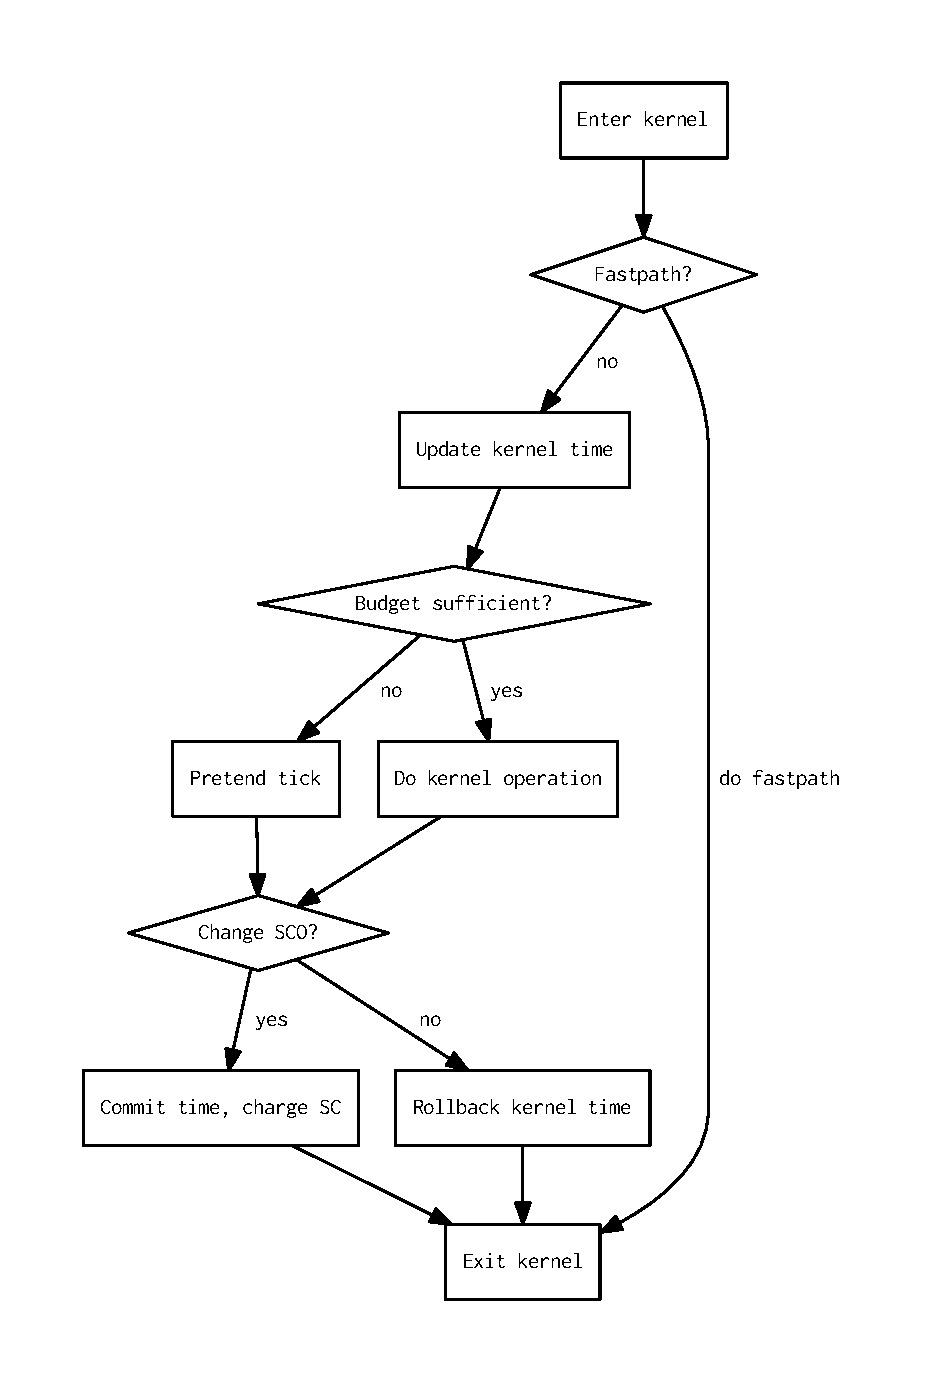
\includegraphics[width=0.8\textwidth]{tickless}
    \caption{Kernel structure}
    \label{figure:tickless}
\end{figure}

\subsubsection{Domain scheduler}

We retain the domain scheduler, as the proof of confidentiality currently requires
it~\citep{Murray_MBGBSLGK_13}, but convert the implementation to tickless, such that domains are
configured with CPU cycles to execute, rather than kernel ticks.

\subsection{Enforcement}

% timeout exceptions, release queue, sporadic servers
The enforcement mechanisms require the most significant changes to the kernel, which we now detail.

The main change required to the existing scheduler is the addition of a \emph{release queue} per
processing core. If a
preempted thread does not have any available replenishments, the kernel removes the thread from the
ready queue to the release queue, retaining the invariant for the ready queue, which the release
queue is characterised as holding all threads that would be runnable but are presently out of
budget. The queue is ordered by the time the next replenishment is available.

\subsubsection{Priority queues}

In addition to the release queue, we also change endpoint and notification object queues
to priority queues, ordered by \gls{TCB} priority. All queues are implemented as ordered, doubly-linked
lists, where all operations complete in $O(1)$ except for insertion, which is $O(n)$, where $n$ 
is the number of threads in the queue. 
We chose the list data structure over a heap for increased performance and reduced verification
burden.

A list-based priority queue out performs a heap-based priority queue for small $n$ in our
implementation up to around $n = 100$.  This $n$ is larger than one would expect in a traditional
\gls{OS}, where heap implementations are array-based in contiguous memory with layouts optimised for
cache usage.  However, because \selfour kernel memory is
managed at user-level (as discussed in \cref{sec:sel4-memory}), data structures must be dynamic, 
resulting in much higher code complexity, and poorer performance than a static heap. 
We do not expect systems to run a large amount of tasks, however if scalability becomes a problem in
practice this implementation could be reconsidered. \citet{Brandenburg:phd} used
binomial heaps for schedulers in \litmus, however Linux does not provide the guarantees, or
implementation requirements of \selfour.

\subsubsection{Timeout Exception Handlers}

Timeout exceptions are only triggered for threads with non-empty timeout handling slots in the
\gls{TCB} \cnode, configured with \tcbsettimeoutep. The implementation is the same as for
fault handlers with one exception: while fault \gls{IPC} messages can trigger scheduling context
donation, allowing fault handling threads to be passive, timeout messages cannot. The timeout
message contains the badge of the scheduling context which triggered the fault, and the amount of
time consumed by that scheduling context since the last reset.

\section{Summary}

In this chapter we have presented the new kernel objects, system call API, invocations and 
structural changes made to provide mechanisms for temporal isolation. 
The implementation adds roughly 2,000 lines of code to \selfour (14\% increase), as measured
by source lines of code (SLOC)~\citep{Wheeler_01} on the pre-processed code for the \textsc{Sabre}, the verified platform.
In the next chapter, we evaluate our implementation with a series of microbenchmarks, 
system benchmarks and case studies.


